\documentclass[polish,polish,a4paper]{report}
\usepackage[T1]{fontenc}
\usepackage[utf8]{inputenc}
\usepackage{babel}
\usepackage{pslatex}
\usepackage{graphicx}
\usepackage{tikz}
\usepackage{pgfplots}
\usepackage{anysize}
\usepackage{pgfgantt}
\usepackage{tabularx}
\usepackage{float}
\usepackage{latexsym,amsmath}
\marginsize{2.5cm}{2.5cm}{3cm}{3cm}

\newcommand{\name}[1]{\sffamily\bfseries\scriptsize #1}

\newcommand{\frontpage}[8]{
%% #1 - nazwa kursu
%% #2 - kierunek 
%% #3 - termin 
%% #4 - temat 
%% #5 - problem
%% #6 - data

\vspace{2cm}

\begin{tabular}{|p{0.72\textwidth}|p{0.28\textwidth}|}
\hline
\multicolumn{2}{|c|}{}\\
\multicolumn{2}{|c|}{{\LARGE #1}}\\
\multicolumn{2}{|c|}{}\\
\hline
\name{Kierunek} & \name{Termin}\\
\multicolumn{1}{|c|}{\textit{#2}} & \multicolumn{1}{|c|}{\textit{#3}} \\
\hline
\name{Imię i nazwisko} & \name{Prowadzący}\\
\multicolumn{1}{|c|}{\textit{#4}} & \multicolumn{1}{|c|}{\textit{mgr inż. Szymon Datko}} \\
\hline
\end{tabular}

}

\usepackage{listings}
\usepackage{xcolor} % for setting colors

% set the default code style
\lstset{ % General setup for the package
	basicstyle=\small,
	numbers=left,
	frame=tb,
	tabsize=2,
	columns=fixed,
	showstringspaces=false,
	showtabs=false,
	keepspaces,
	commentstyle=\color{red},
	keywordstyle=\color{blue}
}

\title{Sprawozdanie Grafika Komputerowa}
\begin{document}
% #1 - nazwa kursu #2 - kierunek  #3 - termin #4 - temat #5 - problem #6 - data
\frontpage{Grafika komputerowa i komunikacja człowiek-komputer}{Informatyka}{Poniedziałek parzysty 11:00}{Patryk Wlazłyń}
\pagestyle{empty}
\newpage

\pagebreak

\setcounter{chapter}{1}
\chapter*{Podstawy \begin{flushright} 28.10.2019 \end{flushright}}

\setcounter{section}{0}
\section{Opis ćwiczenia}
Ćwiczenie polegało na poznaniu elementarnych operacji dostarczanych dzięki standardowi oraz bibliotece graficznej OpenGL. Jako bibliotekę pomocną do 
tworzenia i zarządzania oknami użyliśmy również biblioteki GLUT (GL Utility Toolkit). Podczas tego ćwiczenia poznaliśmy jak zainicjalizować bibliotekę,
jakie są różnice między używaniem jej na platformie Windows oraz Linux oraz jak generować obraz za pomocą wbudowanych prymitywów w przestrzeni 2D.
Naszym głównym zadaniem do wykonania było narysoowanie dywanu Sierpińskiego, zarówno za pomocą algorytmu rekurencyjnego oraz iteracyjnego. Dodatkowo
miał być on zbudowany z bardzo małych, różnokolorowych kwadratów z drobnymi zniekształceniami.

\section{Rozwiązanie rekurencyjne}
Dywan Sierpińskiego składa się z jednego kwadratu w którym wycinane są dziury w postaci mniejszych kwadratów których bok jest dokładnie 3 razy mniejszy i
rozstawione symetrycznie po każdej ze stron (lewo, prawo, góra, dół) oraz pomiędzy nimi, w rogach (górny-lewo, górne-prawo, dolne-lewo, dolne-prawo).
Łatwo zauważyć, że struktura ta powstaje w takim razie w bardzo ścisłym porządku. Ważnym spostrzeżeniem jest też, że wycinania dokonujemy na obszarach
wielkości dokładnie tej samej co środkowy (głowny) kwadrat, lecz każdy z wyciętych kwadratów jest zwyczajnie 3 razy mniejszy. To pozwala na implementacje
trywialnego algorytmu rekurencyjnego polegającego na wycięciu głównego kwadratu w środku aktualnego obszaru a następnie wycięcie mniejszych, ale zwyczajnie
mniejszch, przesuniętych wzgledem głownego o jego szerokość. Taką procedurę wystarczy powrótrzyć dla każdego nowo utworzonego (mniejszego) z kwadratów
dodając dodatkowo maksymalny poziom zagłębienia i otrzymujemy procedurę rekurencyjną generującą dywan Sierpińskiego.

\section{Rozwiązanie iteracyjne}
Rozwiązanie iteracyjne, najłatwiej jest rozwiązać poprzez spojrzenie na gotowy, wygenerowany dywan Śierpińskiego i zauważenie, że "dziury" konkretnych
wielkości rozstawione są w równych odstępach od siebie i występują regularnie na całej powierzchni dywanu. Ważną informacją jest to, że wieksze dziury
wydają się "przykrywać" te mniejsze. Łącząc te dwie informacje otrzymujemy dwie procedury do wykonania, aby narysować dywan. Równomierne pokrycie 
największego kwadratu dziurami oraz należy zacząć od dziur najmniejszych, tak aby te później rysowane (większe) nadpisały obraz wygenerowany przez
wcześniejsze (mniejsze).

\section{Dodatki}
Losowanie koloru zostało osiągniete poprzez losowanie trzech składowych koloru za pomocą funkcji rand z biblioteki standardowej języka C.
Do rysowania kwadratów została użyta funkcja rysująca dwa przystające do siebie trójkąty. Drobne zniekształcenia, wspomniane w opisie, zostały wprowadzone
poprzez losowanie ich zaraz przed narysowaniem kwadratu - funkcja rysująca kwadrat wprowadza zniekształcenia. Podobnie zostało rozwiązane rysowanie
kwadratów kolorowych.

\section{Implementacja - kod źródłowy}
\lstinputlisting[caption=Dywan Sierpińskiego,language=C++]
{class1.cc}

\pagebreak
\section{Zrzuty ekranu aplikacji}
\begin{center}
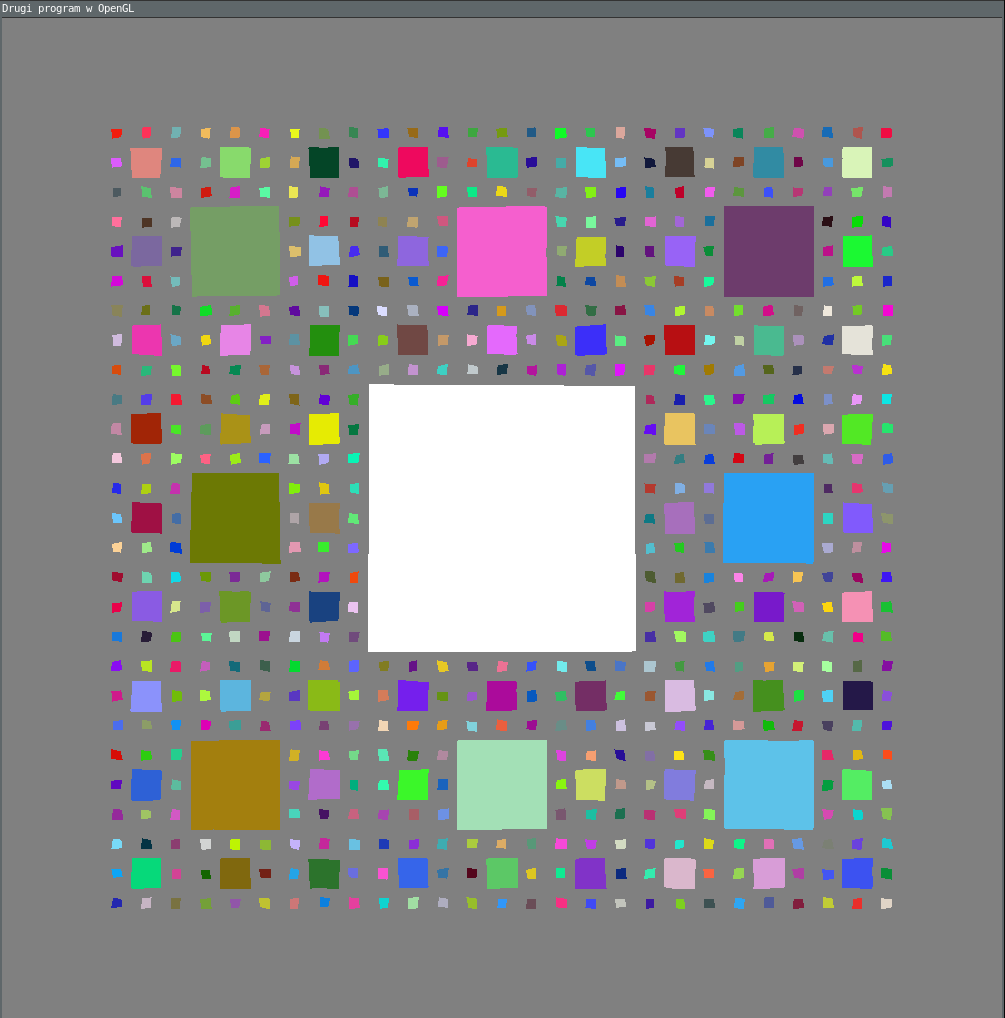
\includegraphics[scale=2]{sierpinski}
\end{center}

\pagebreak
\setcounter{chapter}{2}
\chapter*{Modelowanie obiektów 3-D \begin{flushright} 13.11.2019 \end{flushright}}

\setcounter{section}{0}
\section{Opis ćwiczenia}
Ćwiczenie miało na celu wprowadzenie w zagadnienia związane z modelowaniem i wizualicją scen 3D. Głównymi zagadnieniami przedstawionymi na zajęciach były
transformacje trójwymiarowe na obiektach. Zagadnieniem dodatkowym była obsługa klawiatury do zmiany parametrów animacji. Na ćwiczeniu dane były równanie
otrzymane metodą krzywej Beziera opsujące trójwymiarowy model jajka. Zadaniem autora było narysowanie modelu za pomocą punktów, trójkątów (za pomoca
primitywu GL\_TRIANGLES oraz GL\_TRIANGLE\_STRIP, pokolorowanie oraz włączenie obrotu jajka. Dodatkowo została dodana obsługa klawiatury w celu łatwego
przełączania się pomiędzy trybami wyświetlania.

\section{Rysowanie punktami, oraz siatką}
Po otrzymaniu wzorów które mapują dwu wymiarowe współrzedne na trójwymiarowy punkt rysowanie obiektu jest trywialne.
Podobnie wygląda rysowanie siatki. Wystarczy zmienić tryb rysowania na GL\_LINES.
Poniżej został zamieszczony listing
kodu realizujący to zadanie.

\lstinputlisting[caption=Jajko narysowane punktami,language=C++]
{drawegg_points.cc}

\pagebreak

\begin{figure}[!htb]
\begin{center}
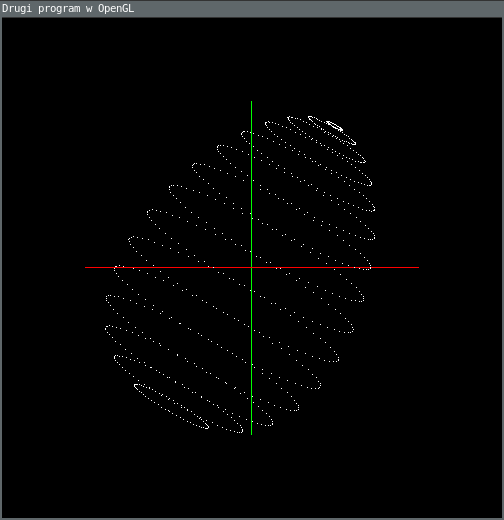
\includegraphics[width=\textwidth]{eggpoints}
\caption{Jajko narysowane za pomocą punktów}
\end{center}
\end{figure}

\pagebreak

\section{Rysowanie trójkątami}
Aby naryswoać jajko za pomocą trójkątów wystarczy ustawić kontekst opengl na rysowanie trójkątami i odpowiednio połączyć sąsiednie punkty, tj.
dla każdego punktu połączyć go z drugim na tym samym poziome, lecz następnego wzdłuż osi X, oraz zamknąc trójkąt łącząc z punktem bedącym nad pierwszym
punktem. Aby jajako składało sie z ładnie przystających trójkątów warto zaraz po tym wykonać juz pierwszy ruch kolejnej iteracji rozpocząć rysowanie
od punktu przesuniętego od początkowego o jeden zarówno w osi X oraz Y. Dzięki obiekt zostanie pokryty idealnie przystającymi trójkątami.
Poniżej został zamieszczony listing kodu realizujący tą funckję.

\lstinputlisting[caption=Jajko narysowane punktami,language=C++]
{drawegg_triangles.cc}

\pagebreak

\begin{figure}[!htb]
\begin{center}
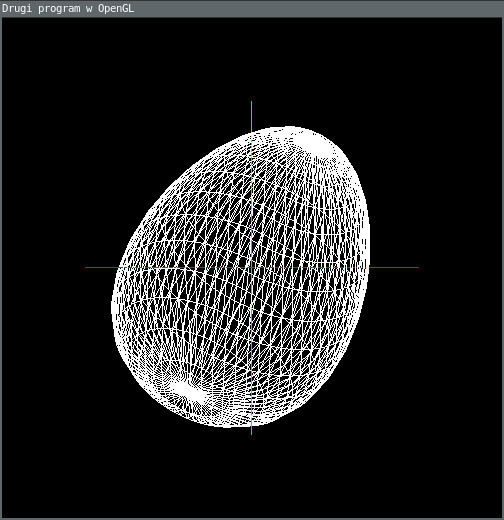
\includegraphics[width=\textwidth]{eggtriangles}
\caption{Jajko narysowane za pomocą trójkątów}
\end{center}
\end{figure}

\pagebreak

\section{Kolorowanie jajka}
Kolorowanie jajka losowymi kolorami odbywa sie poprzed wygenerowanie analogicznej tablicy do tej z zapisanymi punktami, ale tym razem z kolorami dla
każdego koloru, a następnie pobierać ten kolor w czasie rysowania. Inicjalizacja tablicy oraz funckje odpowiedzialne za narysowanie jajka zostały
przedstawione poniżej. Do rysowania użyto prymitywu GL\_TRIANGLES\_STRIP.

\lstinputlisting[caption=Jajko narysowane punktami,language=C++]
{drawegg_tricolo.cc}

\pagebreak

\begin{figure}[!htb]
\begin{center}
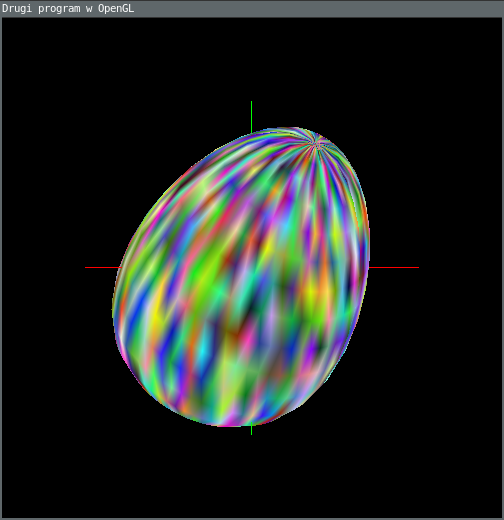
\includegraphics[width=\textwidth]{eggcolor.png}
\caption{Pokolorowane jajko na losowe kolory}
\end{center}
\end{figure}

\pagebreak

\section{Obsługa klawiatury, zmiana parametrów w czasie wykonania}
Aby dodać funckję służącą za obsługę klawiatury należało posłużyć się funkcją z biblioteki GLUT - glutKeyboardFunc(). Jak argument przyjmuje ona wskaźnik
na funkcję, która zostanie wywołana z argumentem jako wciśnięty klawisz (przekonwertowany już na literę ASCII), oraz współrzędne położenia kursora myszy.
Listing opisanych funkcjonalności znajduje się poniżej. Z listingu zostały usuniętę nie istotne fragmenty kodu.

\lstinputlisting[caption=Obsługa klawiatury,language=C++]
{c2_keyboard.cc}

\pagebreak
\setcounter{chapter}{3}
\chapter*{Interakcja z użytkownikiem \begin{flushright} 25.11.2019 \end{flushright}}

\setcounter{section}{0}
\section{Opis ćwiczenia}

\end{document}

